\section{Mask R-CNN} \label{sec:mask_rcnn}

In 2017, the Mask R-CNN model was introduced, which enhanced the Faster R-CNN model and enabled instance segmentation by adding a new branch called the mask branch \cite{mask_rcnn_2017}. The mask branch predicts a binary mask for the object in each proposed RoI on a pixel-by-pixel basis. The mask branch works in parallel with the $reg$ and $cls$ branches of the Fast R-CNN model, which were described in Sec. \ref{sec:fast_rcnn}. In addition to the mask branch, Mask R-CNN also introduces the RoIAlign layer, which projects proposed RoIs onto the feature map and downsamples them to the input size requirement of the next layer \cite{mask_rcnn_2017}. The RoIAlign layer replaces the RoIPool layer to achieve the same functionality without the quantization issue.

\begin{figure}[!ht]
    \centering
    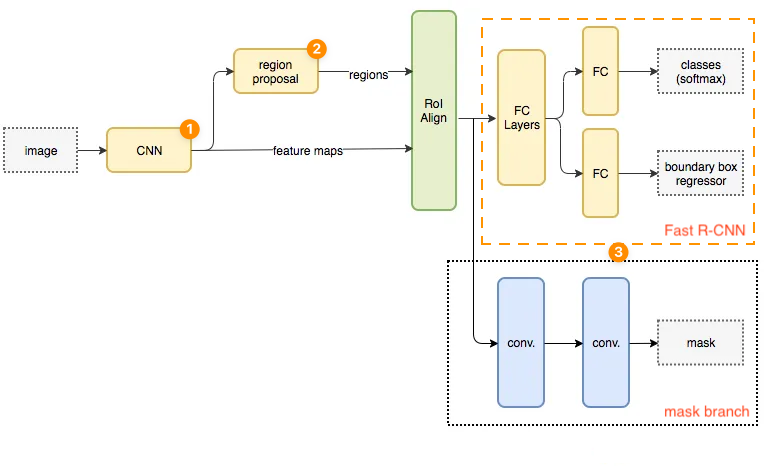
\includegraphics[width=5in]{figures/mask_rcnn_flowc.png}
    \caption{Mask R-CNN network flow \cite{rcnn_vari_flow_chart}} \label{fig:mask_rcnn_flowc}
\end{figure}

The Mask R-CNN architecture consists of three main components (Figure \ref{fig:mask_rcnn_flowc}). These components are a backbone network, a region proposal network (RPN), and the Fast R-CNN model with the addition of a mask branch. The backbone network is a convolutional neural network (CNN) that generates the image's feature map by performing feature extraction on the input image. The second component, RPN, takes the image's feature map as input and generates RoI proposals as described in Sec. \ref{sec:faster_rcnn}. These proposals are then fed into the Fast R-CNN model with a mask branch to predict the classification, the bounding box location, and a binary mask for the object that lies inside each RoI proposal. 

\subsection{The Backbone Convolutional Neural Network}

\begin{figure}[!ht]
    \centering
    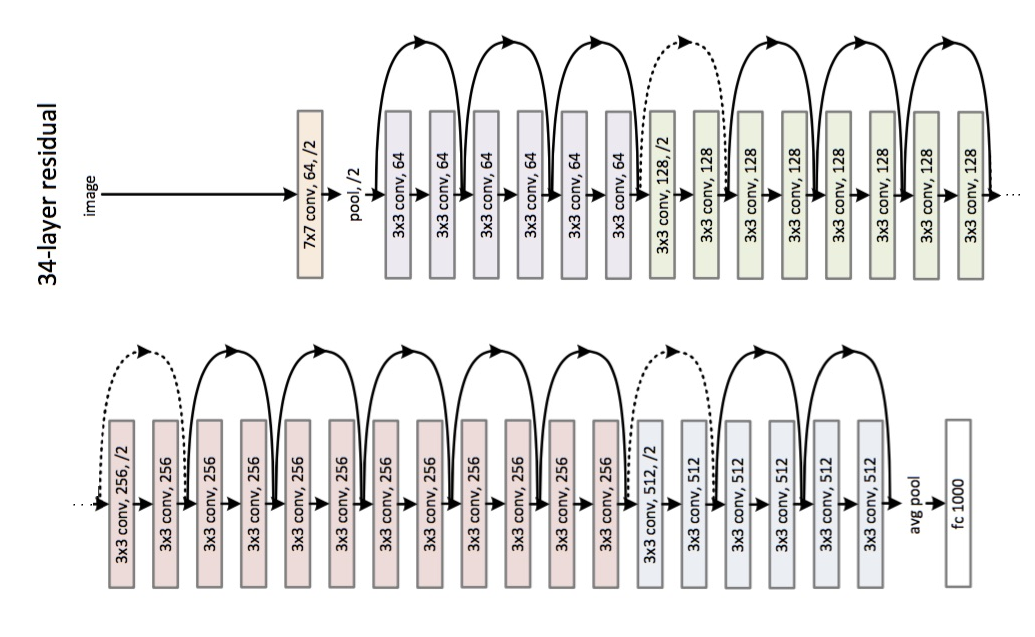
\includegraphics[width=6in]{figures/resnet34_archite.png}
    \caption{ResNet34 overall architecture \cite{resnet_2016}} \label{fig:resnet_archite}
\end{figure}

Similar to its predecessor, the backbone CNN used to generate feature maps within the network model can be any deep CNN like AlexNet and VGG16. The backbone CNN used for Mask R-CNN in the original paper is the ResNet model. There are different implementations of ResNet with varying numbers of layers, including a 34-layer structure depicted in Fig. \ref{fig:resnet_archite}. Like other CNN models, ResNet uses multiple convolutional layers, mostly $3 \times 3$, for feature extraction. ResNet then employs both max-pooling and average-pooling layers for downsampling. ResNet also utilizes a fully connected layer with 1000 neurons for classification. However, this fully connected layer will be dropped to fit with the implementation of Fast R-CNN as described in Sec. \ref{sec:fast_rcnn}. As an important note, ResNet was the first network to introduce the use of identity shortcut connections, which further improve the runtime and address problems with high-depth networks. These connections skip over certain convolutional layers based on certain conditions. The detail of identity shortcut connection remains outside the scope of this paper but can be learned more at He et al., \cite{resnet_2016}. The feature map generated by ResNet34 will then be passed to the RPN and the RoIAlign layer.

\subsection{The RoIAlign Layer}

The RPN generates a list of RoIs on the input feature map as described in Sec. \ref{sec:faster_rcnn}. It is important to note that the RPN does not necessarily ensure that the proposed RoIs will completely cover an exact natural number of feature map pixels, as it is only concerned with the existence of an object at any given location in the feature map. Following this, the feature map RoI proposal and the feature map produced by the backbone CNN are passed to the RoIAlign layer. 

Recall the RoIPool layer from Fast R-CNN; the layer is responsible for mapping proposed RoI of varying to the feature map and downsampling them to a fixed predefined size by performing max-pool operations, described in Sec. \ref{sec:fast_rcnn}. One issue of RoIPool is it is required to perform quantization because it needs the RoI bins in the RoI feature grid to perfectly cover a natural number of pixel in order to perform a max-pooling operation on the feature map pixel value, which lie in each RoI bin. During its operation, the RoIPool layer performs quantization twice. The first quantization happened when the RoIPool map proposed RoIs onto the feature map. The second quantization happens when RoIPool performs downsampling by dividing the RoI feature grid into the RoI bin. These quantizations cause the extracted features to be offset from the input image features, and the model loses a small number of pixels of data for each proposed RoI. While it is acceptable for the object detection model as missing some pixels does not affect the general location and size of the object, pixel offset, and pixel loss have a large negative effect in instance segmentation task, where the model has to identify all pixels belonging to the object.

\begin{figure}[!ht]
    \centering
    \subfloat[][4 regularly spaced points in an RoI bin]{ 
        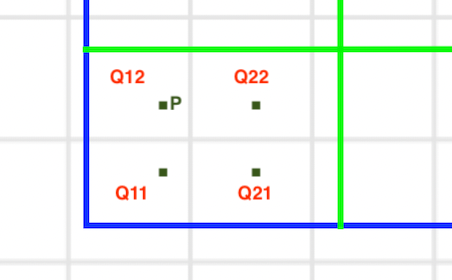
\includegraphics[height=2in]{figures/regularly_point.png}
    }
    \subfloat[][Bilinear interpolation point $P$]{ 
        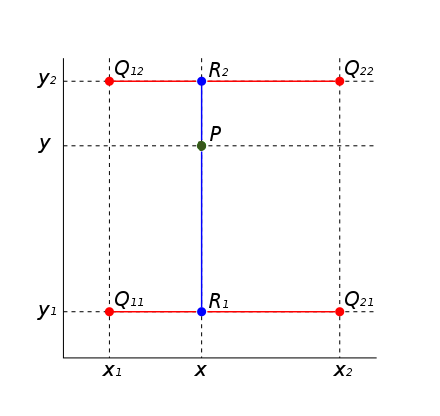
\includegraphics[height=2in]{figures/bilinear_interp_coord.png}
    }
    \caption{\textbf{(a)} A feature map RoI bin, represented by blue and green boundary. The dark green points inside the bin are regularly spaced points. $Q_{ij}$ represents the center of a feature map pixel, which has a coordinate and a feature pixel value. $Q_{11},\ Q_{21},\ Q_{12},\text{ and } Q_{22}$ are the four nearest feature map pixel to point $P$.}
    \label{fig:bin_w_regularly_points}
\end{figure}

Similar to RoIPool, RoIAlign is a layer that aligns a proposed RoI onto a feature map and downsamples the feature map RoI to a predefined size. However, RoIAlign does not have the quantization issue that RoIPool has because it uses max-pooling on the bilinear interpolation value of four regularly spaced points in each RoI bin rather than the feature map pixel value \cite{mask_rcnn_2017}. This means that RoIAlign does not need to use complete pixels to perform the max-pool operation, eliminating the need for quantization. To achieve this, RoIAlign divides the feature map RoI into a grid of equal-sized RoI bins and calculates the location of the four regularly spaced points in each RoI bin. The number of RoI bins along the width and height of the RoI feature map is predefined by the input size requirement of the next layer in the network. With the calculated RoI bins, the four regularly spaced points are located at $(\frac{W}{3}, \frac{H}{3})$, $(\frac{2 \times W}{3}, \frac{H}{3})$, $(\frac{W}{3}, \frac{2 \times H}{3})$, and $(\frac{2 \times W}{3}, \frac{2 \times H}{3})$ in each RoI bin, where $W \times H$ be the size of the RoI bin [Fig. \ref{fig:bin_w_regularly_points}]. Bilinear interpolation is then used to calculate the value of each point based on the four nearest feature map pixels. Let the four nearest feature map pixels to a regularly spaced point $P$ at $(x, y)$ are $Q_{11},\ Q_{21},\ Q_{12},\ Q_{22}$ at $(x_1, y_1),\ (x_2, y_1),\ (x_1, y_2),\ (x_2, y_2)$, respectively, as shown in Figure \ref{fig:bin_w_regularly_points}. Then the bilinear interpolation value of point $P$ can be calculated based on linear interpolation over $x-$coordinate and then $y-$coordinate as follow:

\leftskip1cm\relax
\rightskip1cm\relax
\noindent Let linear interpolation over $x-$coordinate be:
\begin{align*}
    f(R_1) = f(x, y_1) &= \left( \frac{x_2-x}{x_2-x_1}f(Q_{11}) + \frac{x-x_1}{x_2-x_1}f(Q_{21}) \right) \\
    f(R_2) = f(x, y_2) &= \left( \frac{x_2-x}{x_2-x_1}f(Q_{12}) + \frac{x-x_1}{x_2-x_1}f(Q_{22}) \right)
\end{align*}
\noindent Then, the bilinear interpolation of point $P$ can be computed by performing linear interpolation over $y-$coordinate of the linear interpolation result over $x-$coordinate. 
\begin{align}
    f(P) &= \frac{y_2-y}{y_2-y_1} f(R_1) + \frac{y-y_1}{y_2-y_1} f(R_2) \nonumber \\
    &= \frac{y_2-y}{y_2-y_1} f(x, y_1) + \frac{y-y_1}{y_2-y_1} f(x, y_2) \nonumber \\
    &= \frac{y_2-y}{y_2-y_1} \left( \frac{x_2-x}{x_2-x_1}f(Q_{11}) + \frac{x-x_1}{x_2-x_1}f(Q_{21}) \right) \nonumber \\
    &\ \ + \frac{y-y_1}{y_2-y_1} \left( \frac{x_2-x}{x_2-x_1}f(Q_{12}) + \frac{x-x_1}{x_2-x_1}f(Q_{22}) \right) \label{eq:binlinear_interpolation}
\end{align}
\leftskip0cm\relax
\rightskip0cm\relax

\noindent Since the bilinear interpolation technique is based on the value of the four nearest pixels and weights them accordingly based on their location relative to point $P$, it gives RoIAlign a smooth way to estimate the value at point $P$ without shifting. Similarly, the bilinear interpolation value for the other three regularly spaced points in each RoI bin is calculated. With the value of the four regularly spaced points, RoIAlign performs a max-pool operation on these points to choose a value to represent the RoI bin. RoIAlign repeats this process for all RoI bins in the feature map RoI, thus resulting in a fixed predefined output matrix.

\begin{figure}[!ht]
    \centering
    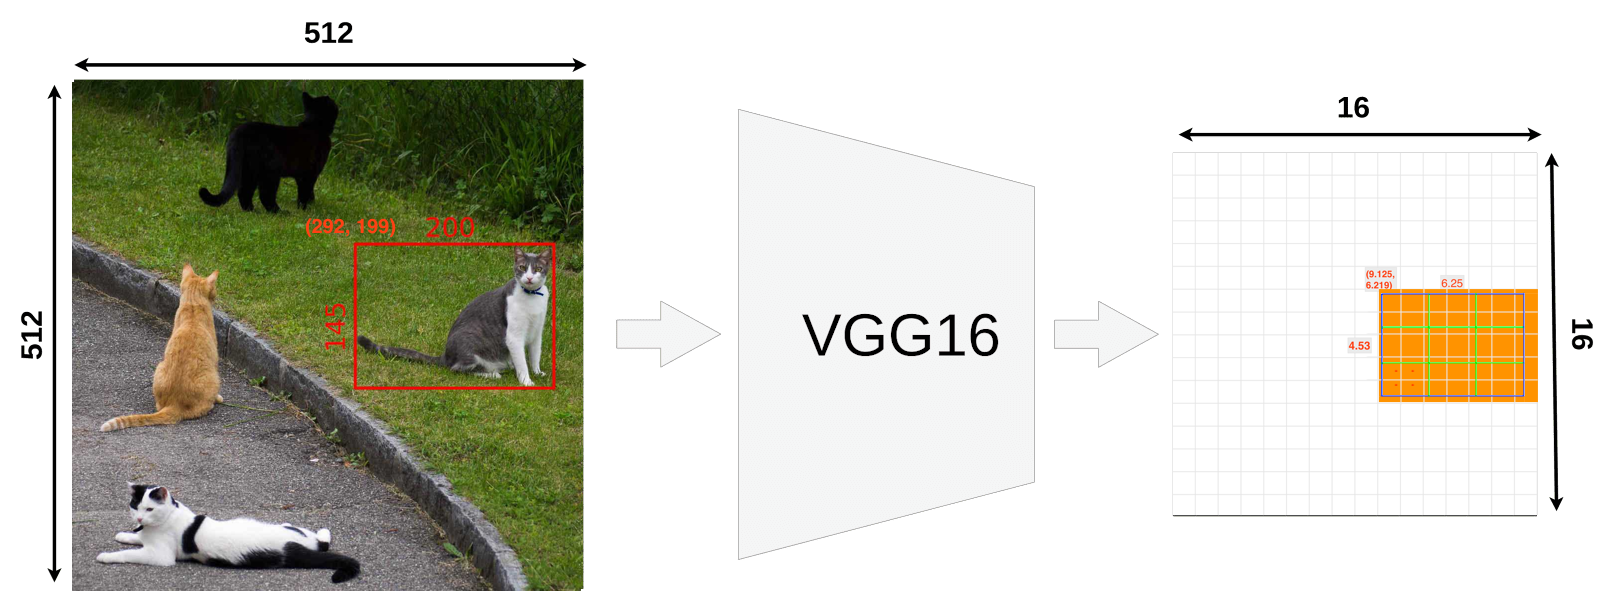
\includegraphics[width=6in]{figures/roi_align_ex.png}
    \caption{Mapping the proposed RoI onto the feature map using RoIAlign. The RoI (red rectangle) on the image space (left) aligns with the proposed RoI (blue rectangle) on the feature map space (right). The rectangles bounded by green or blue borders inside the feature map RoI are RoI bins. The four red dots inside each RoI bin represent the four regularly spaced points for max pool operation. \cite{roi_pooling_problem}}
    \label{fig:roi_align_ex}
\end{figure}

Reconsider the example mentioned in Sec. \ref{sec:fast_rcnn}, we process an image of size $512 \times 512$ image with Mask R-CNN without the mask branch and with VGG16 as the backbone CNN. This setup is the same setup as mentioned in the Fast R-CNN model except for replacing the RoIPool layer with the RoIAlign layer and using RPN to generate RoI proposals. By using RoIAlign, the proposed RoI location is the same between the input image and the image feature map [Fig. \ref{fig:roi_align_ex}]. Furthermore, when downsampling the feature map RoI, RoIAlign does not lose information like RoIPool. Instead, RoIAlign uses bilinear interpolation on each point inside each RoI bin and samples from the surrounding feature map pixels. While both layer output a $3 \times 3$ matrix for each proposed RoI, in our example RoI proposal, RoIPool only sample $6 \times 3$ feature map pixels, $1.67$ times smaller compared to $6 \times 5$ feature map sampled by RoIAlign [Fig. \ref{fig:roi_align_ex}, Fig. \ref{fig:roi_projection_ex}, and Fig. \ref{fig:roi_pool_ex}]. This allows the RoIAlign layer's output matrix to convey more information and helps maintain the required input size for the next layer.

\begin{figure}[!ht]
    \centering
    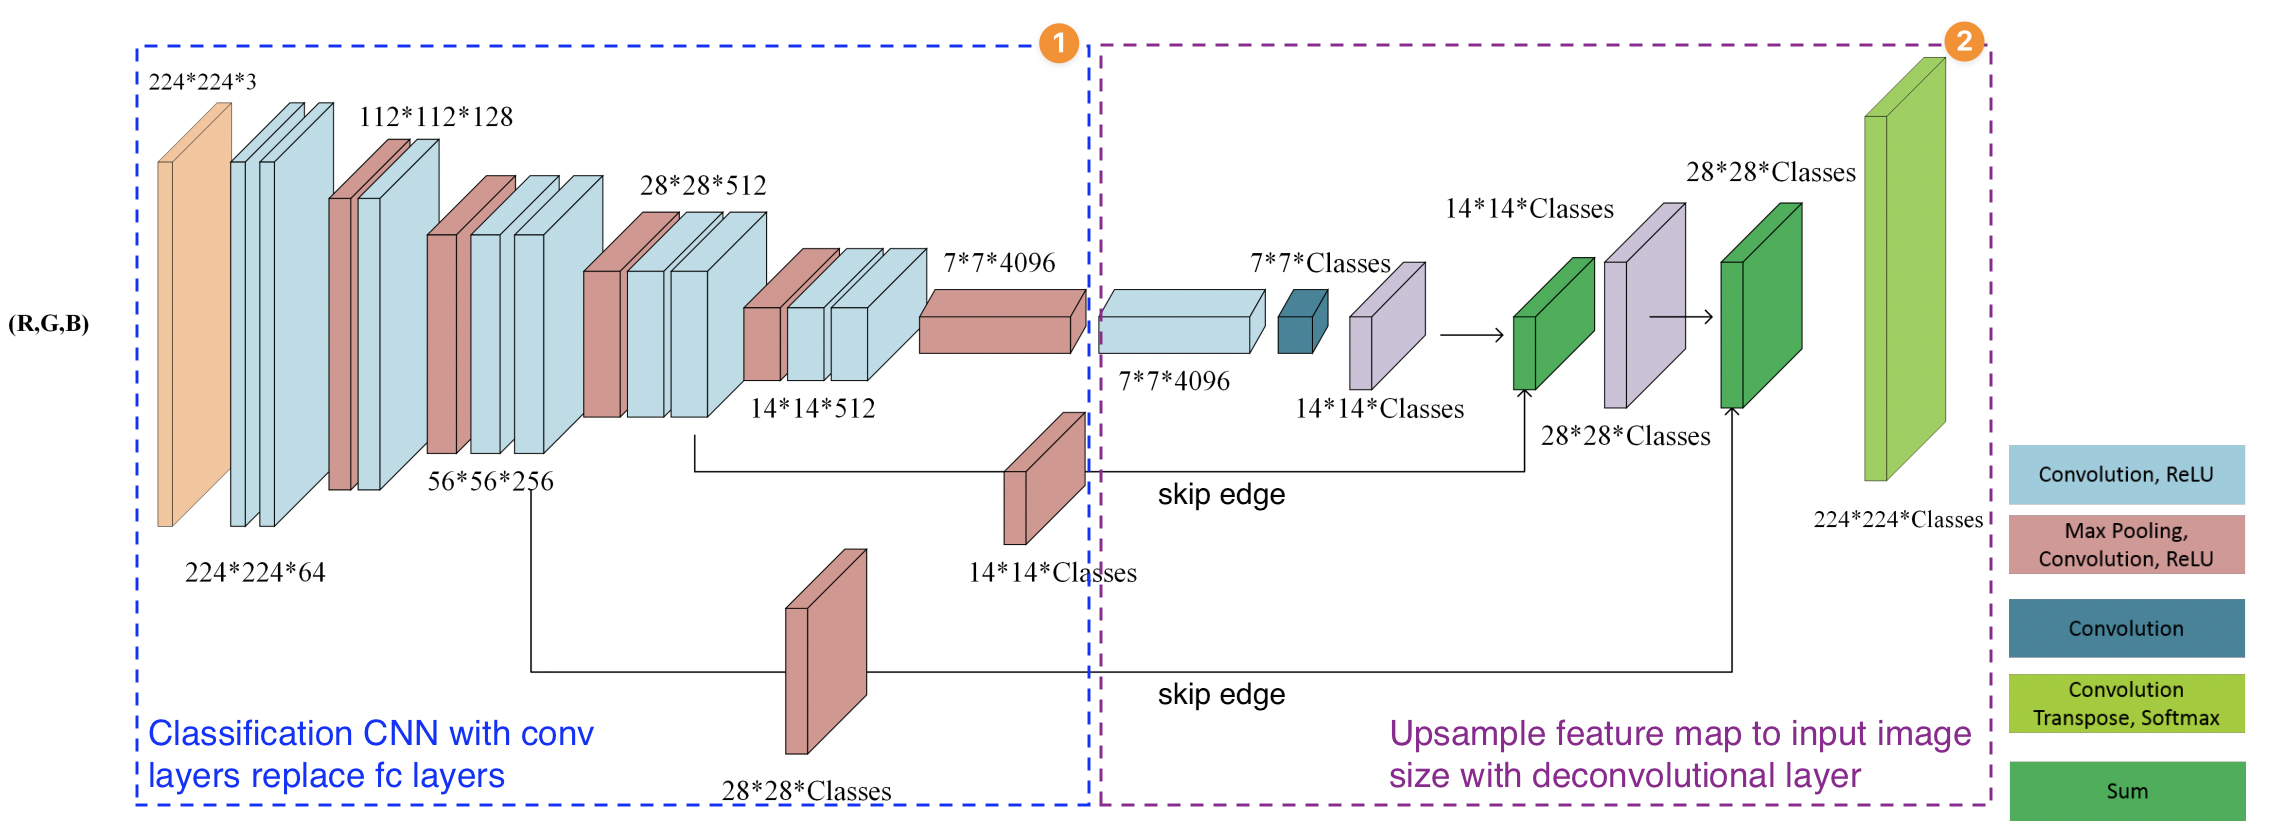
\includegraphics[width=5in]{figures/fcn_archite.png}
    \caption{Fully Convolutional Network (FCN) with stride 8 \cite{fcn_archite_2018}} 
    \label{fig:fcn_archite}
\end{figure}

\subsection{The Mask Branch}

Additional to the RoIAlign layer, Mask R-CNN introduces a mask branch running parallel with the bounding box regressor branch and classification branch as included in the Fast R-CNN model \cite{mask_rcnn_2017}. The mask branch is based on a fully convolution neural network, which was first proposed for the semantic segmentation task. We will use FCN as the acronym for the fully convolution network, as opposed to the fully connected network, for the remainder of this section. 

The FCN model is based on the classification CNN model, like AlexNet and VGG16, with the ability to predict classification for each pixel in the image \cite{mask_rcnn_2017}. The FCN overall architecture consists of two stages [Fig. \ref{fig:fcn_archite}]. The first stage is known as an encoder. The encoder is responsible for downsampling the input image and generating a feature map along with classification for each feature map pixel. Similar to the traditional classification CNN, the encoder can generate a feature map with a set of convolutional layers. In a classification CNN, once the feature map is generated, a fully connected layer will be used to classify the object in the feature map, which introduces two problems to the network. The first problem is the network will lose the spatial location of all feature map pixels. This is because the feature map must be flattened to a 1-dimensional matrix of size $n_1 \times 1$, where $n_1$ is the number of neurons in the first fully connected layer, to convert the feature map to a fully connected layer. Then the first layer's neurons connect and activate the second layer's neurons by performing a matrix multiplication with the transposed weight matrix of size $n_1 \times n_2$, where $n_2$ is the number of neurons in the second fully connected layer. That is $[n_1 \times n_2]^T [n_1 \times 1] = [n_2 \times 1]$, thus correctly resulting in the second fully connected layer with a dimension of $n_2 \times 1$. However, due to fully connected layer matrix multiplication, these layers are required to have a fixed size. Thus resulting in the second problem of the fully connected layer is required the network to have a fixed input size. The issue of fully connected layers is not desired in the encoder network as it must maintain the spatial location of all feature map pixels so that the decoder can upsample the subsampled (encoded) feature map. Recall equation \ref{feature_size_eq}, which use to calculate the feature size after applying a convolution layer. Assuming the kernel size is equal to the layer's input feature map and we do not use zero-padding, then the network's layer will result in a feature map of size $1 \times 1$. By applying $n_1$ kernels where each kernel has the same size as the layer's input feature map, the network will achieve the same $n_1$ neurons. This is the same as when using a fully connected layer but removes the shortcoming of losing spatial information \cite{mask_rcnn_2017}. Therefore, the encoder part of FCN is able to perform feature map generation and feature map pixel classification without the loss of pixels' spatial location by replacing the fully connected layers with convolution layers in a traditional classification CNN.

\begin{figure}[!ht]
    \centering
    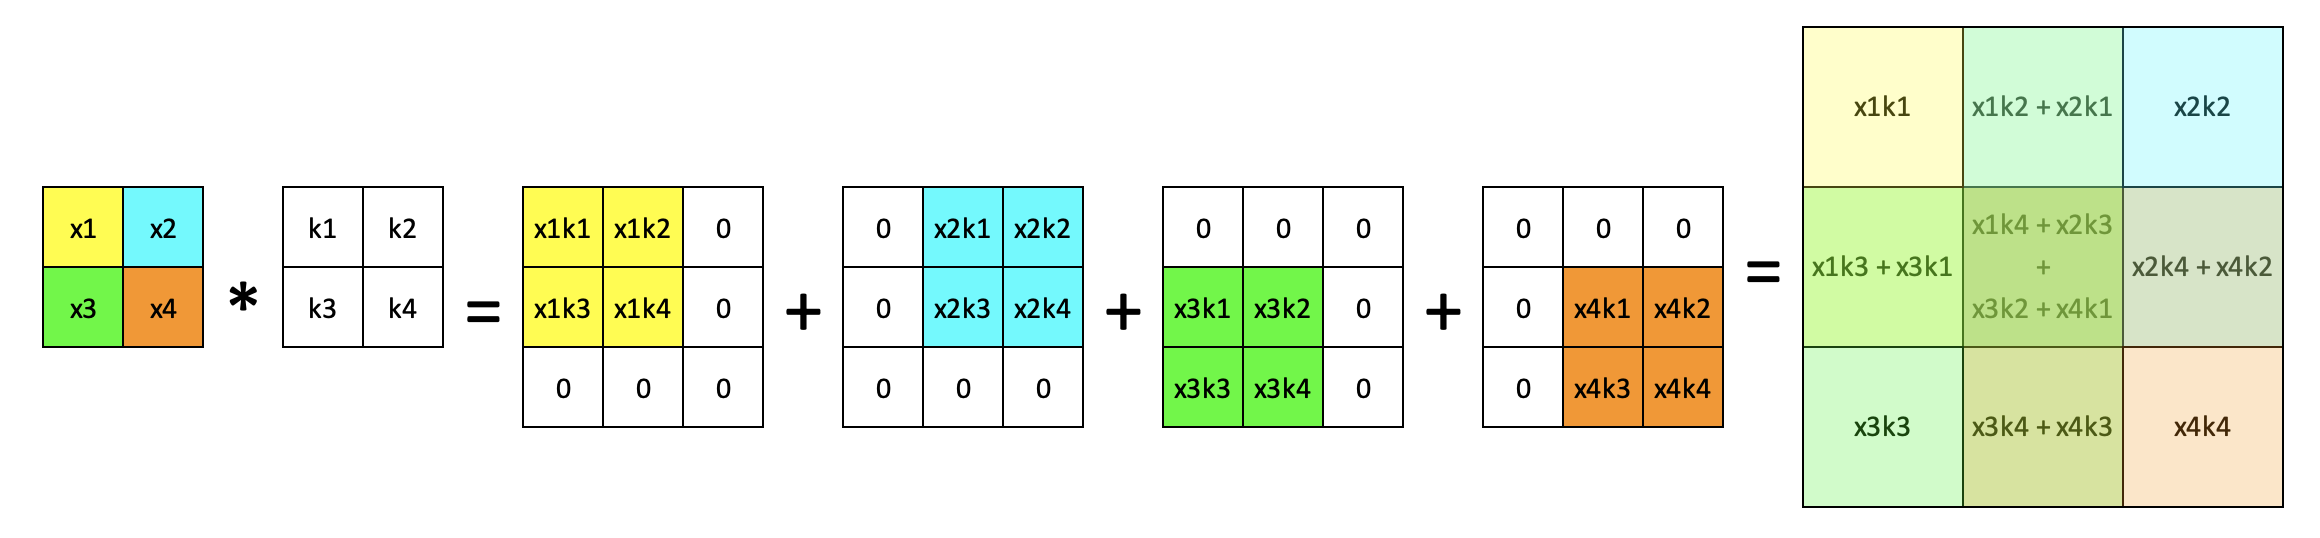
\includegraphics[width=5.5in]{figures/transpose_convo1.png}
    \caption{Apply $2 \times 2$ upsample learnable kernel, with stride of 1 and no zero-padding, on a low resolution feature map. Result of the upsampled operation is a $3 \times 3$ feature map.}  \label{fig:transpose_convo}
\end{figure}

With the spatial location and class label of all pixels in the feature map generated by the encoder, the decoder, the second stage of the FCN model, can upsample these classified feature map pixels to the input image space. By upsampling the classified pixel, the decoder will be able to project objects' pixel-wise mask from the feature map space to the input image space. The decoder performs the upsampling operation by using the learnable transposed convolution layer, also known by other names like fractionally strided convolution, backward strided convolution, or upconvolution \cite{transposed_convolution_layer_2016}. When upsampling an input feature matrix, the transpose convolution layer first applies a learnable kernel to each element of the input matrix by performing scalar matrix multiplication \cite{mask_rcnn_2017}. The learnable kernel has it's weight randomly initialized or with an upsampling technique like bilinear interpolation. The location of the multiplicated matrix on the output matrix is determined by the kernel size and stride. That is the result of our scalar matrix multiplication between the input matrix element and kernel matrix, which will slide on the output matrix with the stride of $\floor{\frac{1}{f}}$, where $f$ is the scale factor between the input image and output image. Note that if our kernel size is larger than the kernel stride, then the multiplicated matrix is overlapping with one another on the output matrix, and thus we concatenate the overlapped cell of these multiplicated matrices together. An example of an overlaping transpose convolution layer is shown in Figure \ref{fig:transpose_convo}, where kernel size is 2 and stride is 1. Additionally, transposed convolution is responsible for negating the size change of the convolution operation; thus we can invert the Equation \ref{feature_size_eq} to see the relationship between kernel size, kernel stride, and zero padding interact with one another as follow:
% 
% The decoder, which is the second stage of the FCN model, can upsample the classified feature map pixels generated by the encoder to the input image space using the spatial location and class label of all pixels in the feature map. This enables the decoder to project objects' pixel-wise mask from the feature map space to the input image space. To perform the upsampling operation, the decoder uses a learnable transposed convolution layer, which is also referred to as fractionally strided convolution, backward strided convolution, or upconvolution \cite{transposed_convolution_layer_2016}. When upsampling an input feature matrix, the transposed convolution layer first applies a learnable kernel to each element of the input matrix through scalar matrix multiplication. The learnable kernel can be initialized with random weights or using an upsampling technique such as bilinear interpolation. The location of the multiplicated matrix on the output matrix is determined by the kernel size and stride. Specifically, the scalar matrix multiplication between the input matrix element and kernel matrix results in a sliding window operation with a stride of $\floor{\frac{1}{f}}$, where $f$ is the scale factor between the input image and output image. If the kernel size is larger than the kernel stride, the multiplicated matrix overlaps with one another on the output matrix, and we concatenate the overlapped cells of these matrices together. Figure \ref{fig:transpose_convo} illustrates an example of an overlapping transpose convolution layer with a kernel size of 2 and stride of 1. Additionally, the transposed convolution is responsible for negating the size change of the convolution operation. Thus, we can invert Equation \ref{feature_size_eq} to see how the kernel size, kernel stride, and zero padding interact with one another.
%
$$\text{output size} = \text{input size} - 1 \times \text{kernel stride} - 2 \times \text{zero-padding size} + \text{kernel size}$$
Let's consider the example of upsampling a $2 \times 2$ feature map to the image size of $32 \times 32$, which corresponds to a scale factor of 16. Without using any zero-padding, the kernel size must be $32 - (2-1) \times 16 = 16$ for both the width and height of the kernel. The FCN model that performs a scale factor of 16 after downsampling for classification is referred to as FCN-16s. In the original FCN paper, the authors proposed three variations of the FCN model: FCN-32s, FCN-16s, and FCN-8s. The architecture of the FCN-8s model is illustrated in Figure \ref{fig:fcn8_archite}.

\begin{figure}[!ht]
    \centering
    \subfloat[][The FCN-8s architecture \cite{fcn_archite_2018}]{ 
        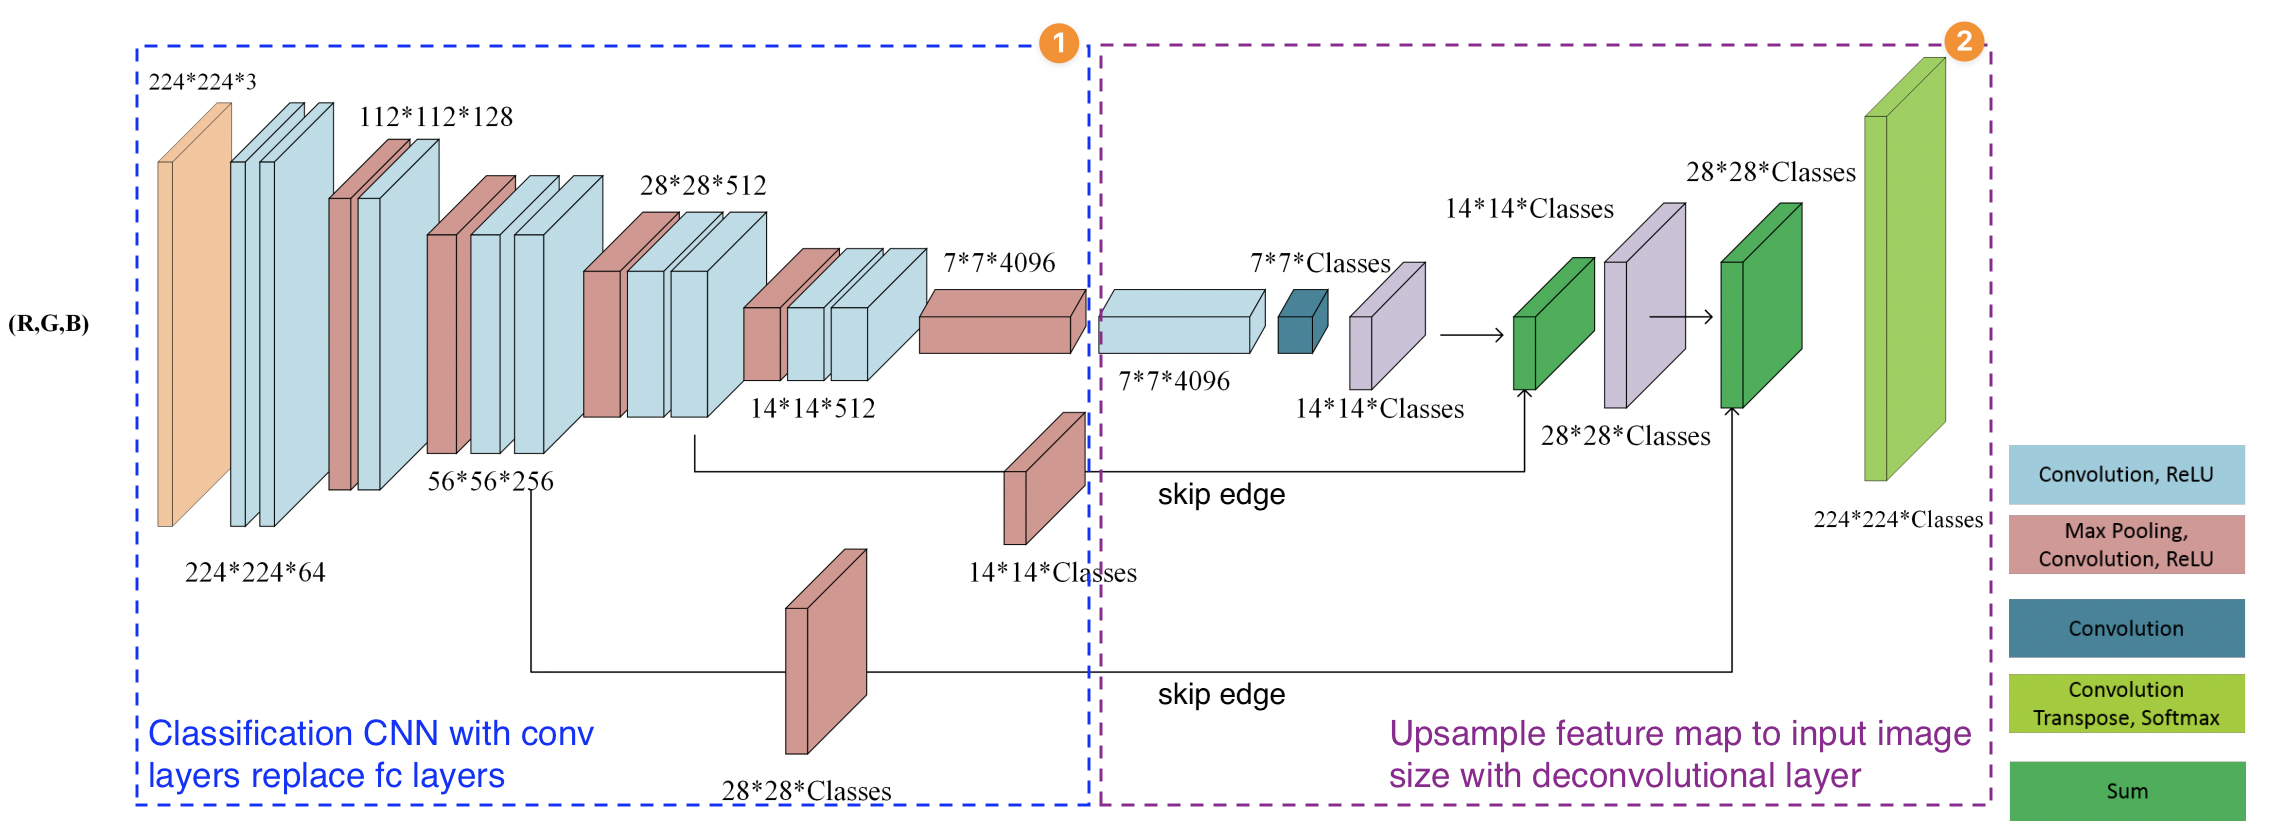
\includegraphics[width=5in]{figures/fcn_archite.png} \label{fig:fcn8_archite}
    }

    \subfloat[][The output mask for different versions of the FCN model. The $n$ in the FCN-ns name denotes the upscaling factor of the model. As we can see, FCN-32s has the lowest resolution as the model upscales the image by 32 times. On the other hand, the FCN-8s has a higher resolution as the upscaling factor is 8 times, which is possible with the use of skip connections.]{ 
        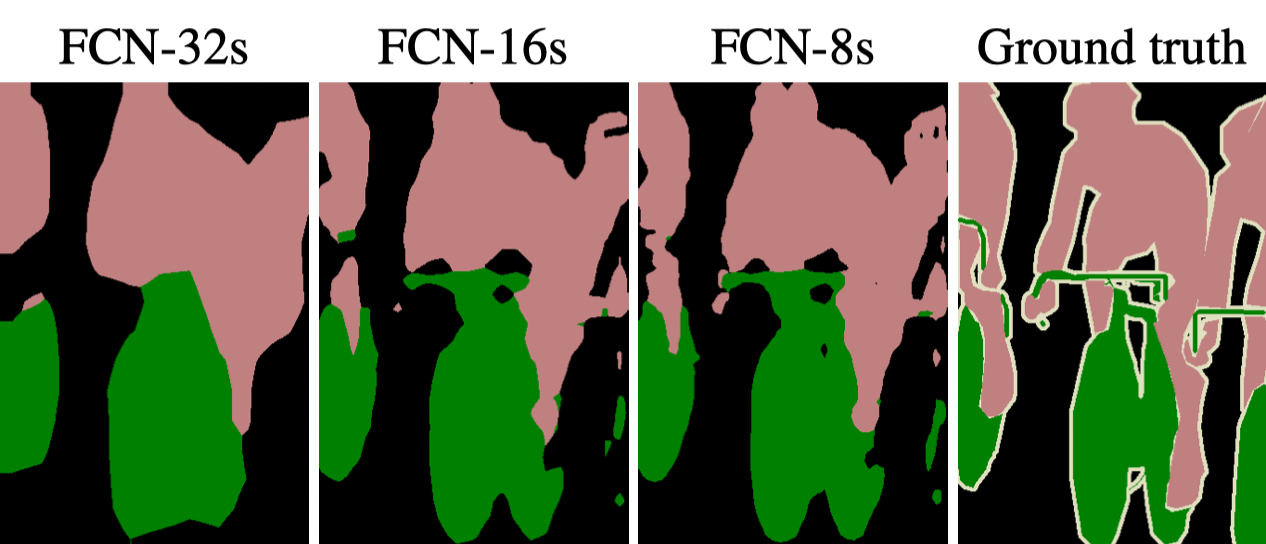
\includegraphics[width=5in]{figures/fcn_output_mask.png} \label{fig:fcn_output_mask}
    }
\end{figure}

The skip connection is a key element in improving the accuracy of segmentation masks produced by Fully Convolutional Networks (FCN). As seen in Figure \ref{fig:fcn_output_mask}, while FCN-32s can provide a rough idea of object locations, it has low pixel accuracy. To address this issue, FCN-16s and FCN-8s use skip connections and reduce the scale factor, as shown in Figure \ref{fig:fcn_skip_conn}. The skip connection allows the FCN to retain the original feature map before downsampling, which is then concatenated with a classified upsampled feature map of the same size \cite{mask_rcnn_2017}. This process reduces the scaling factor needed for upsampling and enables the original feature map to contribute to predicting missing pixels. With the additional information from the skip connection, the FCN can project the classified pixels more accurately onto the denser space, resulting in improved segmentation masks.

\begin{figure}[!ht]
    \centering
    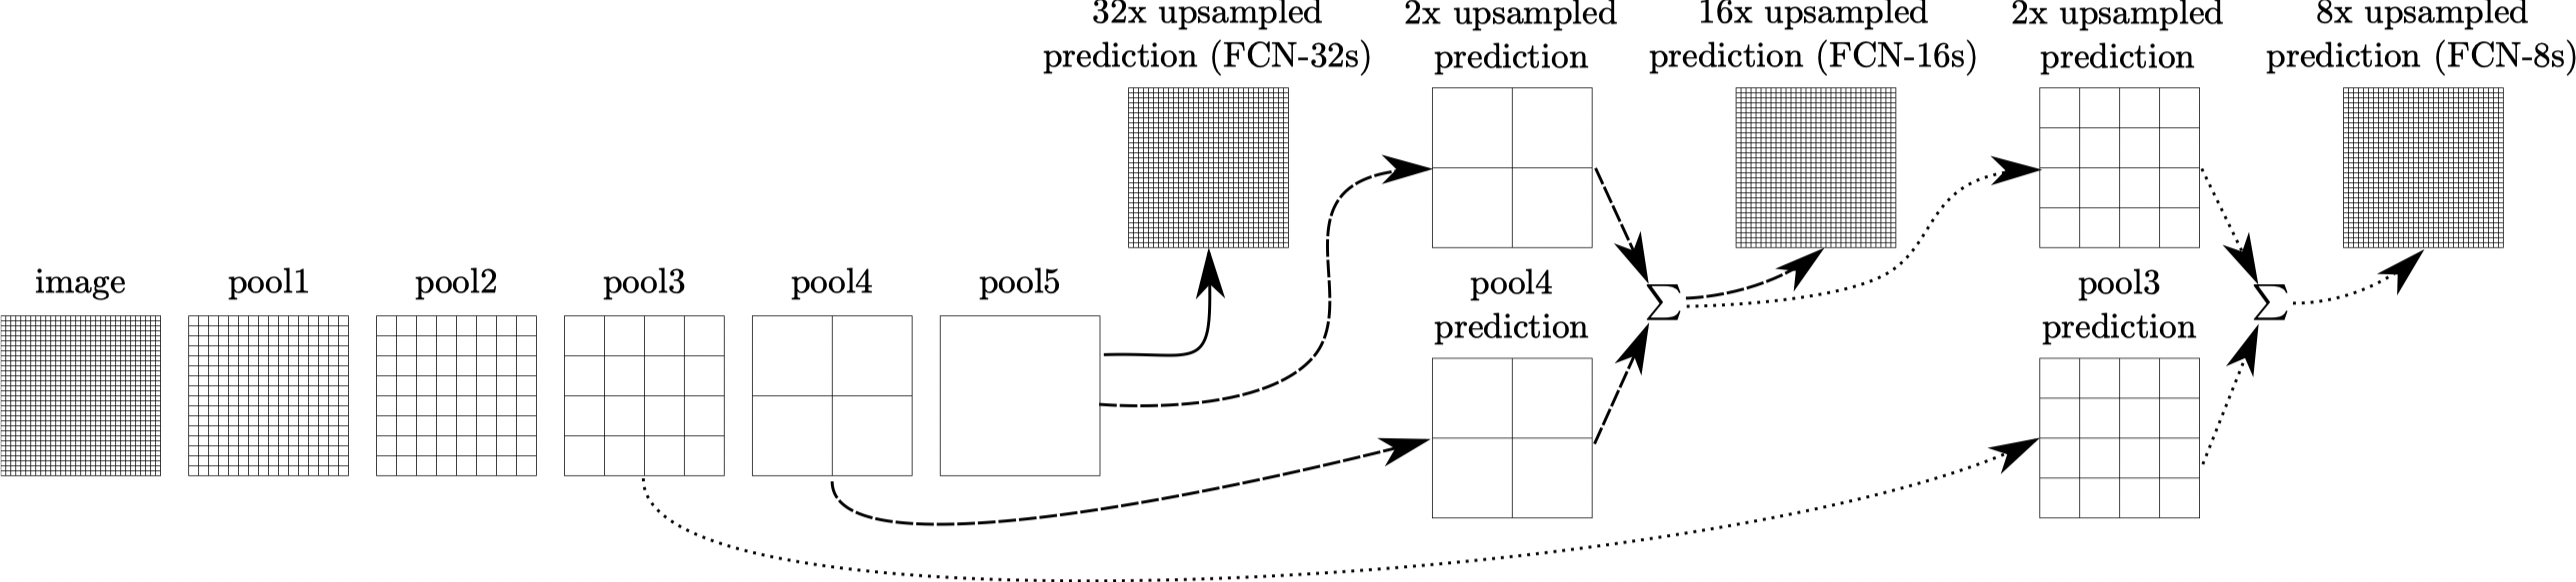
\includegraphics[width=6in]{figures/fcn_skip_conn.png}
    \caption{{\color{red} FCN skip connection}}  \label{fig:fcn_skip_conn}
\end{figure}